\chapter{Thermal Convection Loop Experiment}
\chaptermark{Thermosyphon} %this is the chapter heading that will show on subsequent pages

The thermosyphon, a type of natural convection loop or non-mechanical heat pump, can be likened to a toy model of climate \shortcite{harris2011predicting}.

\section{Thermal Convection Loops}

Under certain conditions, thermal convection loops covect operate as non-mechanical heat pumps, making them useful in many applications.
As mentioned in the introduction, 

\section{Ehrhard-M\"{u}ller Equations}

Following the derivation by Harris \shortcite{harris2011predicting}, itself a representation of the derivation of Gorman \shortcite{gorman1986} and namesakes Ehrhard and M\"{u}ller \shortcite{ehrhard1990dynamical}, I derive the equations governing the thermosyphon.

Similar to the presented derivation of the governing equations of CFD in Chapter 3, I start with a small but finite volume inside the loop.
Here, however, the volume is described by $\Delta \pi r^2 \Delta R \delta \phi$ for $r$ the interior loop size, $R$ the $\phi$ the angle within and for the whole loop, respectively.
The second law states that momemtum is conserved, such that the sum of the forces acting upon our finite volume is equal to the momemtum of this volume.
Therefore we have the basic starting point for forces $F$ and velocity $u$ as
\begin{equation*} \sum F = u \rho \pi \Delta r^r \Delta R \Delta \phi \end{equation*}

\todo{finish up}

\section{Detailed Experimental Setup}

Originally built (and subsequently melted) by Dr. Chris Danforth, the University of Vermont's current experimental thermosyphons have made considerable progress.
Operated by Dave Hammond, UVM's Scientific Electronics Technician and master parameter tuner, the experimental thermosyphons access the chaotic regime of state space found in the principled governing equations.

\todo{include real timeseries, if possible}

\begin{figure}[tpb!]
  \centering
  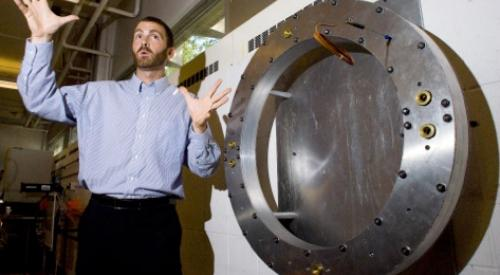
\includegraphics[width=0.49\textwidth]{figures/danforth.jpg}
  \caption{
  Professor Chris Danforth with the Thermal Convection Loop.
  }
  \label{fig:chrisLoop}
\end{figure}
\todo{photo permission??}






